%!TEX root = ../main.tex
%%=====================================================================
%%  §5  THE COROLLARY: THE FIELD CONVERGES      target 4-5 pp.
%%
%%  Four cuts, each holding more fixed, then the aggregation corollary.
%%  The venue audit's note: this reads as a failed horse race and is
%%  actually an IDENTIFICATION result. Write it that way -- the question
%%  is what a downstream Sharpe ratio can resolve about the clustering.
%%
%%  6.0  *** THE STRONGEST EVIDENCE FOR THIS SECTION'S TITLE ARRIVED
%%       2026-08-15 AND IS NOT YET IN THE PLAN BELOW. CORRECTIONS.md N22.
%%
%%       Changing the SEED of one algorithm rearranges nearly as much of
%%       the partition as changing the algorithm entirely. Verified twice,
%%       independently, on the partition files alone -- no head run, no
%%       CUDA, nothing to reproduce:
%%
%%         same method, different partition seed   mean ARI 0.4229
%%         different method, same seed             mean ARI 0.1945
%%         => a seed rearranges (1-0.4229)/(1-0.1945) = 0.72 of what an
%%            algorithm change rearranges
%%         (compute branch measured 0.767 on its own sampling; agree)
%%
%%       agglo_avg and agglo_complete return ARI 1.0000 across seeds --
%%       deterministic, as expected. random returns ~0.000 -- independent
%%       draws, as expected. Both controls behave, which is what makes the
%%       0.42 for the stochastic methods meaningful.
%%
%%       AND THE RANKING FLIPS. On the naive layer, which is deterministic
%%       and reproduces to 16 digits, so the spread is PURE partition-seed
%%       effect:
%%         kmeans_ret  1.8961 / 2.0342 / 1.9745   (ps42/ps1/ps123)
%%         pca_load    1.9142 / 1.8135 / 1.9977
%%         spectral    1.7119 / 1.6604 / 1.6747
%%       Two of three seeds put pca_load first, one puts kmeans_ret first
%%       by 0.2208. pca_load's own partition-seed range (0.1842) is 91% of
%%       the across-method range at ps42 (0.2023). The BOTTOM is stable --
%%       spectral is last at all three.
%%
%%       ⚠ CAVEATS TO CARRY, all three stated by the compute branch:
%%         (a) NAIVE layer. The tournament headline is the trained head's,
%%             and the naive layer's own ranking differs (agglo_complete
%%             leads it). So this is a strong prior, NOT yet a statement
%%             about the tournament. GPU arms queued.
%%         (b) n = 3 partition seeds.
%%         (c) head seed pinned at 42, so the design traces an "L" through
%%             the 3x3 grid: both MARGINALS, never the interaction. ⛔ Do
%%             not run a seed-replicate ANOVA assuming additivity without
%%             saying the interaction was never estimated.
%%
%%       ⛔ WITHDRAW, wherever it appears: "kmeans_ret leads and is the
%%          most stable in the field, std 0.0152". That 0.0152 is the
%%          HEAD-seed s.d.; its partition-seed s.d. is 0.0693, 4.6x
%%          larger. Restate as "most stable across head-training seeds"
%%          or drop it. AUDIT.md:50 and :250 are superseded.
%%
%%  6.1  ⚠ THE POOLED YARDSTICK IS DEFINED HERE NOW, not in §3. It moved
%%       when §4 was folded into §3 on 2026-08-15, because it is a tool
%%       for THIS section's claim and belongs where it is used. §3.5
%%       already points forward to it. One paragraph, and it must carry:
%%         - a per-arm s.d. from three draws is not a yardstick: its own
%%           95% interval spans a factor of six
%%         - so pool: 0.1354 on 39 residual d.f. over 19 arms / 58 runs
%%         - AND PRINT THE YARDSTICK'S OWN INTERVAL, chi-square
%%           [0.1109, 0.1739]. A difference of "1.2 pooled s.d." is 1.0 or
%%           1.5 depending where the true ruler sits; the reader needs
%%           that margin to read the adjacency claim.
%%         - ⚠ SCOPE (§3.5): this measures HEAD-TRAINING variation, since
%%           the partition is byte-identical across seeds. It answers
%%           "would a different training run reverse this ordering" and
%%           NOT "would a different partition draw reverse it". The second
%%           question has no answer in this design outside SSSNET.
%%       ⚠ ARM-SET CONFLICT, unresolved: NUMBERS.md N4.2 gives 0.1354
%%         over 19 arms; the common-window field of
%%         _reference/NEWSTATS_common_window_field.md gives 0.1194 over
%%         12 methods + 2 controls. Name the set in the sentence.
%%
%%  6.1  THE FIELD. Twelve methods, two controls, three seeds each.
%%       Adjacent differences are inside the pooled yardstick (§4.3).
%%       ⚠ Restrict any rank assertion to a COMMON ESTIMATION WINDOW.
%%       ⛔ NOT "correlation window" -- k-means on returns builds no
%%          correlation matrix at all (KMeans on Rtr.T, 60 raw residual
%%          features, no corrcoef in its path), so the phrase is false for
%%          that arm. Eleven of twelve build C over the window and for
%%          them the two phrases coincide. Provenance audit 2026-08-15.
%%       Within the five native 60-day methods the span is 0.5286.
%%       ⛔ No adjacent-pair ordering claim, anywhere.
%%
%%  6.2  HOLD THE METHOD, CHANGE ONLY THE INPUT WINDOW.
%%       *** REWRITTEN 2026-08-15 to N20/N21. The previous version of
%%       *** this block quoted t = 68.0, which CORRECTIONS.md N20(c)
%%       *** forbids outright. See EVIDENCE.md §6 for the full grid.
%%
%%       Complete grid: 5 methods x 4 windows x 3 seeds = 60 runs, all
%%       6,941 days, all gate-passing. Delta(252-21), paired by seed:
%%         spectral_unsigned +0.7945 (p=0.019)   pca_load +0.5883 (0.0097)
%%         sponge            +0.4105 (p=0.045)   agglo_complete +0.2394
%%                                                  (p=0.091, UNRESOLVED)
%%         agglo_avg         +0.0102 (flat)      kmeans_ret -0.0007
%%
%%       LEAD WITH THE DIFFERENCE-IN-DIFFERENCES, not the per-method
%%       deltas. agglo_avg, pca_load and spectral_unsigned consume the
%%       IDENTICAL object C = np.corrcoef(Rtr.T) and differ only in how
%%       they read it, so a difference between their window responses
%%       cannot be a panel, universe, book or era effect:
%%         pca_load - agglo_avg          +0.5780  p = 0.027
%%         spectral_unsigned - agglo_avg +0.7843  p = 0.0010
%%       both sign-consistent across all three seeds.
%%
%%       MECHANISM: window sensitivity tracks whether a method reads the
%%       EIGENSTRUCTURE of C, not whether it consumes C. The a-priori
%%       reason is the BBP threshold -- at N~490 a population eigenvalue
%%       must exceed sqrt(N/T) to be recoverable: 4.83 at T=21 (only the
%%       market mode survives) against 1.39 at T=252 (sector-scale modes
%%       survive). Rank deficiency alone would predict all five methods
%%       suffer at w21, which is NOT observed.
%%
%%       BOOK INVARIANCE holds for THREE arms only -- pca_load 0.0014%,
%%       agglo_complete 0.0021%, spectral 0.0026%. agglo_avg moves 0.158%
%%       and kmeans_ret 0.615%, so the general statement is false.
%%
%%       RESOLVED 2026-08-16 night: the discriminating experiment
%%       REPORTED and the rival is falsified on all three pre-registered
%%       arms (spot-verified against recomputed SRs). The concession
%%       sentence is REPLACED by the result in §5.5; do not restore
%%       "better motivated story, not the better supported one".
%%       Mechanism survives on classification+direction, understates
%%       magnitude (+0.59 predicted vs +0.91 observed, pca_load@K50).
%%
%%       ⛔ NEVER QUOTE: t = 68.0, or N21's t = 30.96 -- both are
%%          degenerate denominators (three paired diffs with sd 0.0056
%%          and 0.0439). QUOTE THE EFFECT SIZE, NEVER THE t.
%%       ⛔ spectral's span is 0.7945, NOT 0.8067 (that came from a w60
%%          cell computed on two seeds).
%%       ⛔ "the only significant window result in the campaign" -- false.
%%       ⛔ "one input parameter moves one method further than the
%%          algorithm choice moves the field" -- WITHDRAWN. Paired by
%%          seed it reverses on 2 of 3 seeds; bootstrap P = 0.63, CI
%%          [-0.22, +0.23].
%%       ⛔ "extremes vs averaging" -- the properly controlled test
%%          (agglo_avg vs agglo_complete) gives +0.2292, p = 0.28, not
%%          sign-consistent. Dead.
%%       ⛔ kmeans_ret as an averaging or window-unused control. The
%%          window is its FEATURE DIMENSION and rearranges its partition
%%          as much as anyone's (ARI(w21,w252) = 0.143).
%%       ⛔ kmeans_ret "shows no window effect". Write "not
%%          distinguishable from zero, CI +/-0.41".
%%       ⛔ Do NOT write that 60 is optimal because it matches the beta
%%          window. That hypothesis was proposed and falsified.
%%
%%  6.2b THE K SWEEP -- partial, 22 of 60 in as of 2026-08-15.
%%       pca_load is CLEAN: +0.4552 across K=10..40 with the traded book
%%       moving 0.006%.
%%       kmeans_ret is CONFOUNDED: its K effect is collinear with a
%%       4.17% shrink of the traded book, corr(SR, book) = -0.93
%%       (p = 0.023), both monotone in K. The channel is
%%       SPONGE_MIN_CLUSTER_SIZE = 2 -- singletons rise from 1.42 to
%%       23.05 per day and are deleted. "More clusters" and "trades
%%       fewer names" are NOT SEPARABLE in this design. Say so.
%%
%%  6.2c ONE SENTENCE ONLY -- the table lives in the appendix.
%%       Effective K spans 8.07 to 28.93 across arms nominally set to
%%       thirty, and it does NOT explain the ordering:
%%       Spearman(K_eff, SR) = -0.24, p = 0.44 (AUDIT.md §F).
%%       So the reflex objection -- "some partitions are simply better,
%%       you ranked on the wrong dimension" -- is foreclosed by the data
%%       rather than argued with. Point at the appendix table and move on.
%%       ⛔ Do NOT reproduce the size table here, and do NOT add a
%%          sentence defending the random control; the numbers do it.
%%
%%  6.3  HOLD THE METHOD AND THE WINDOW, CHANGE ONLY THE SEED.
%%       The learned-graph method's three seeds give partitions no more
%%       similar to each other (ARI 0.1583/0.1594/0.1612) than to a
%%       different method entirely (0.1532/0.1569/0.1554), yet their
%%       Sharpe range is 0.2434. This is the cleanest cut: even the
%%       algorithm is held fixed.
%%
%%  6.4  HOLD EVERYTHING, CHANGE THE ERA. Individual configurations move
%%       a great deal in rank -- the k-means arm travels from 1st to 3rd
%%       to 14th to 15th of 24 -- while the OVERALL ordering is preserved
%%       (Spearman +0.7333/+0.6281/+0.8105/+0.7105 against the full
%%       sample, nineteen configurations, seed-averaged convention).
%%       ⛔ Print no rank without its field size. "1 -> 2 -> 7 -> 7" is a
%%          field-of-twelve statement and was printed unlabelled.
%%       ⛔ "The full-sample ordering reproduces in no sub-period after
%%          2001" is FALSE. And the affirmative form is equally
%%          forbidden -- it is the retired exhibit in the other direction.
%%
%%  6.5  WHAT INFERENCE RESOLVES. Model confidence set at 90% retains 9
%%       of 12 (T_max); report BOTH statistics, since T_R retains 3 at
%%       the rule-based layer and reporting either alone is a choice of
%%       answer rather than a result. Ledoit-Wolf pairwise: 7 of 66
%%       survive Holm, none adjacent. The Sortino/Sharpe twin pair --
%%       identical in every hyperparameter, the study's only clean
%%       objective contrast -- is a NULL: +0.0874, s.e. 0.0989, p = 0.38.
%%       ⚠ THE ANNUALizATION RESULT, and both halves must be printed
%%       together: sqrt(252) is arm-dependent (corr with the 21-day
%%       correction = -0.92) and STRETCHES the field. On non-overlapping
%%       21-day sums the twelve-method spread falls 0.5522 -> 0.2155,
%%       below its own noise band, a 75% confidence set retains ALL
%%       TWELVE, and 0 of 66 pairs survive Holm. What survives everything:
%%       every method beats both floors.
%%       ⛔ Quoting either half alone is forbidden, and so is the converse
%%          overreach that the ranking is pure noise -- 330 observations
%%          failing to reject is not proof.
%%
%%  6.6  COMBINING, as the corollary. Selection on past performance and
%%       equal weighting are INDISTINGUISHABLE (true only for the
%%       expanding-window rule that selection loses; all three rolling
%%       rules win, all insignificantly). Equal weight 2.6664 reaches
%%       99.17% of the equal-weighting limit 2.6887.
%%       ⛔ That limit is the n->infinity limit of EQUAL weighting of
%%          exchangeable streams. It is NOT a bound over arbitrary
%%          weightings -- a top-k subset reaches 107.23% of it.
%%
%%  FIGURES: fig_window_twin, fig_cum_pnl, fig_select_vs_ew.
%%=====================================================================
\section{Comparing the Clusterizers}
\label{sec:invariance}
%% RETITLED 2026-08-15 night. Under the hedge-vs-signal thesis this
%% section's negative results are PREDICTIONS: if what a clustering
%% delivers downstream is mainly a hedge, and the twelve rules remove
%% nearly the same amount of comovement (17.5-20.2% (full-window, corrected 2026-08-16), §4), then their
%% books should be statistically inseparable -- and they are. Write the
%% section in that order: prediction first, then the four cuts as
%% confirmations, then the noise ledger (N22) as the reason ranking was
%% never going to resolve.

This section compares the 12 clusterizers against the variation the design itself produces when a training run or a partition draw is repeated. Their partitions disagree, yet the books they produce move together, and their Sharpe ratios separate the top of the ranking from the bottom without separating neighbors in the middle. \secref{sec:field} measures how far the gap between two clusterizers moves when only the training run changes, and uses that dispersion as the benchmark for the ranking. \secref{sec:pseed} redraws the seed behind each partition and finds that the leader of the ranking depends on the draw. \secref{sec:formal} runs the formal tests. \secref{sec:gradient} follows the differences between clusterizers at three points along the pipeline, from the partition to the payoff, and draws the consequence for choosing among them. \secref{sec:window} turns to the two inputs that do move the results, the estimation window and the number of groups.

\subsection{Variation across Training Runs}
\label{sec:field}

Most adjacent gaps in the Sharpe ranking are smaller than the run-to-run
variation in the gap itself. A ranking compares two arms, so the dispersion a
gap must be judged against is the dispersion of the difference between them,
not of either arm's level. The two are not interchangeable here, and the reason
can be measured. In the $12 \times 5$ matrix of per-seed Sharpe ratios, $27\%$
of the variance is a shift shared by every arm: a seed that trains one
configuration well trains all 12 well. The five seed means span $0.41$,
half the $0.83$ between the best and the worst clusterizer. A shared shift
moves every arm together and can reorder nothing. Only the interaction between
arm and seed can, and it carries $8\%$ of the variance.

Pooled across the 11 adjacent pairs, the standard deviation of a gap across its
five training runs is $0.103$, on 44 degrees of freedom, with a $95\%$ interval
of $[0.085, 0.130]$. Measured on the levels instead, the dispersion is $0.168$
on 48 degrees of freedom, a fifth of the span between the best and the worst clusterizer. We report
both and judge the gaps against the paired figure, which is the error term a
comparison across a common set of seeds calls for.\footnote{This is a different
safeguard from the data-snooping corrections of \citet{white2000reality},
\citet{hansen2011mcs}, and \citet{bailey2014deflated}, which take each measured
statistic as given and protect a comparison against selection across many
tests. The dispersion measured here is the statistic's own run-to-run noise, so
the two safeguards are complements.}

The 12 mean-of-per-seed Sharpe ratios span $1.742$ to $2.567$, and nine of the
11 adjacent gaps are smaller than $0.103$; the count is eight at the interval's
lower end and nine at its upper. Both exceptions sit at the ends of the
ranking. $k$-means on returns leads the second clusterizer by $0.139$, and
\textsc{gics} leads spectral clustering at the bottom by $0.245$, the only gap
that also exceeds the dispersion of the levels. The nine gaps between them run
from $0.001$ to $0.090$.

Even the separation at the top does not fix the leader. $k$-means on returns is
first at four of the five seeds and complete linkage at the fifth. Only the
bottom of the ranking is fixed: spectral clustering is last at every seed. The
ordering is therefore not expected to replicate between neighbors
(\figref{fig:field_ruler}).

\begin{figure}[tb]
\centering
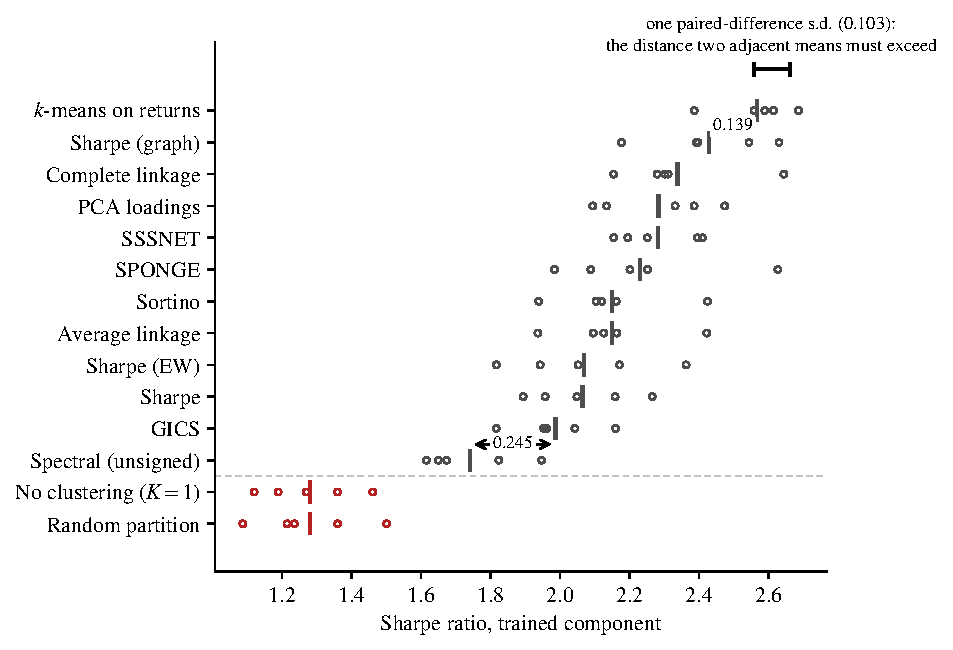
\includegraphics[width=\linewidth]{fig_field_ruler}
\caption{Per-seed Sharpe ratios against the dispersion of a gap. This figure plots
the per-seed Sharpe ratios of the 14 arms at the trained component over the
$6{,}913$-day window. Each row is one arm: circles are its five per-seed Sharpe ratios, the tick its mean. The bar at the top right is not an interval around a
center; its \emph{length} is one pooled paired-difference standard deviation, $0.103$, the distance two adjacent means must exceed, and it is meant to be laid
against the horizontal distance between two neighboring ticks. Nine of the 11
gaps between adjacent clusterizer means fall inside it; the two that do not are
marked, at the top and the bottom of the ranking. Measured on the levels instead the dispersion is $0.168$, and by that wider figure 10 of the 11 gaps fall inside. Both controls sit below every clusterizer run.}
\label{fig:field_ruler}
\end{figure}


\subsection{Variation across Partition Draws}
\label{sec:pseed}

The training-seed dispersion of \secref{sec:field} leaves out the variation in the partition itself. Every stochastic clusterizer's daily partitions were generated once and cached, and all five training runs use the same partitions (\secref{sec:seeds}). Redrawing the partition measures how much that draw moves the results. This subsection is reported on a different basis from the rest of the paper: five partition draws, each traded by a single training run at head seed $42$, so that the partition axis is isolated. The five training seeds of \secref{sec:seeds} do not enter here.

For the nine stochastic clusterizers, each redrawn five times (partition seeds $1$ to $5$; the cached partition of the rest of the paper is a separate draw), the adjusted Rand index (\textsc{ari}; \citealp{hubert1985comparing}) between two draws of the same clusterizer averages $0.30$, against $0.19$ between two different clusterizers. Expressed as disagreement, one minus the index, a redraw of the seed produces $87\%$ of the disagreement that a change of clusterizer produces. The average hides three levels that do not overlap. The four trading-driven clusterizers agree with their own redraw at $0.21$ to $0.28$, the four other stochastic clusterizers at $0.32$ to $0.45$, and \textsc{sssnet} at $0.18$, so stability against the seed is a property of the family.

Redrawing the partition moves the Sharpe ratios as well; the largest range grows from $0.21$ under the fixed rule to $0.38$ under the neural trading head, though not every clusterizer moves more. At the rule-based component, which has no training noise, the draw already moves the leader (\figref{fig:pseed_flip}a): spectral clustering is last under all five seeds, but $k$-means on returns is first under only three of them, Sharpe (graph) and PCA loadings under one each. The largest range across the five draws is $0.21$, for $k$-means on returns, $36\%$ of the $0.58$ between the best and the worst of the 45 rule-based books (nine clusterizers at five partition seeds); the random control, whose labels are redrawn daily under any seed, moves $0.08$.

Under the neural trading head the leader still depends on the draw and the movement is larger. When the head is rerun with its own seed pinned on the same redrawn partitions, $k$-means is first at four of the five draws and \textsc{sponge} at the other. The largest range across the five draws grows by three quarters, to $0.38$ for \textsc{sponge}, and the random control moves $0.39$
(\figref{fig:pseed_flip}b), as much as it moves across the five head seeds ($0.41$, \figref{fig:field_ruler}). The trained component, which might be expected to average the draw away, instead enlarges it, and for a partition that carries no information it converts the draw into as much variation as a refit does. \textsc{sssnet}, redrawn like the others, moves by $0.15$ at the rule-based component and by $0.13$ under the head, the fifth-largest and the smallest ranges among the nine. A ranking computed from one partition draw per clusterizer therefore carries a source of variation that rerunning the training leaves in place and enlarges.
%% ⚠ N84 (2026-09-01): sec:pseed now uses partition seeds {1,2,3,4,5} (head 42 pinned); the two comment blocks below describe the retired {42,1,123} basis. Numbers: repo analysis/results_5seed + figures/scripts/fig_pseed_flip_v3.py (computed from the books).
%% HEAD layer, 9 rules + random, head seed 42, ps{42,1,123}, ALL
%% verified vs run CSVs (2026-08-17 night, jobs 61623872+61637228):
%% kmeans 2.5443/2.6210/2.5784 (range .0767), pca_load
%% 2.3735/2.4243/2.3198 (.1045), spectral 2.2078/2.1632/2.1374
%% (.0704), sponge 2.4413/2.5239/2.2230 (.3009), sharpe_fixed
%% 2.4234/2.4076/2.2996 (.1238), sortino 2.4118/2.3573/2.2137
%% (.1981), fv2a 2.2199/2.2896/2.2259 (.0697), fv3sm
%% 2.5295/2.5803/2.3186 (.2617), random 1.2854/1.3431/1.5874 (.3020).
%% head/rule range ratios: fv2a .46, pca .46, kmeans .67 (damped);
%% spectral 1.39, sharpe_fixed 1.40, fv3sm 1.62, sponge 2.04,
%% sortino 3.94, random 6.81 (amplified).
%% WITHDRAWN on the full sample (do not restore): "the head damps the
%% partition draw" (was true only for the first four arms measured);
%% "random 0.30 is 4x any real rule" (sponge .3009 matches it);
%% "ordering identical under every seed" (true of the leader only).
%% Naive-layer numbers unchanged (paper basis, pseed_naive_paper_basis
%% + pseed_naive_RAW_OOS, cross-validated 4.9e-05).

\begin{figure}[tb]
\centering
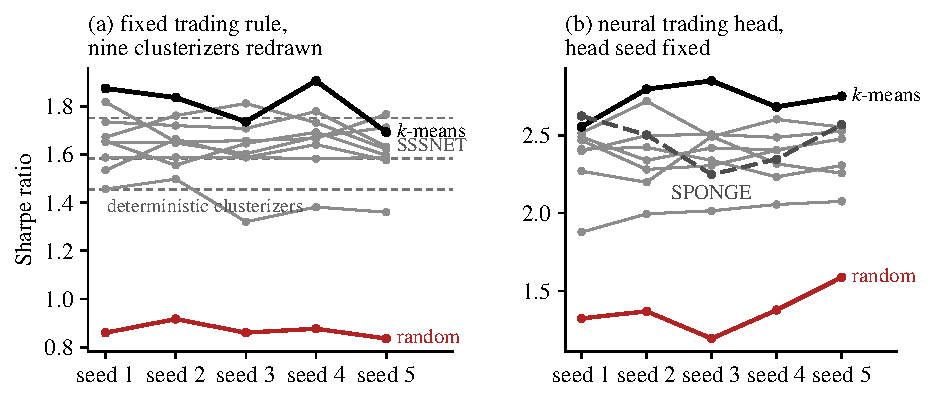
\includegraphics[width=\linewidth]{fig_pseed_flip}
\caption{Redrawing the partition seed at each trading component. This figure plots the Sharpe ratio of each stochastic clusterizer under five partition seeds. The labels on the horizontal axis name those partition seeds, not the training seeds of \secref{sec:seeds}, which are held fixed here. (a)
The rule-based component is deterministic, so every movement is the
partition draw itself. Spectral clustering is last under all five
seeds; $k$-means (black) is first under three of them, and the largest range is $0.21$. The panel tracks the nine stochastic clusterizers; the three deterministic ones, with no seed to redraw, are the dashed horizontals. (b) The trained component, with the head seed pinned at $42$ and the same nine clusterizers. $k$-means (black) is first at
seeds $2$ to $5$, \textsc{sponge} (dashed) at seed $1$. The largest range across the five draws is larger here than at the rule-based component, and so is the random control's. The random control is red in both
panels.}
\label{fig:pseed_flip}
\end{figure}

%%  ⚠ v3/cal6913 SENTINEL (N51-N53; supersedes the N22 block that stood
%%    here -- its naive-flip story and "up to 0.18" were V2 values):
%%    - naive layer: k-means FIRST under all three partition draws
%%      (1.7810/1.8735/1.9213); largest naive redraw range 0.23
%%      (Sharpe (EW), 0.2293); random moves 0.06 (0.0592).
%%    - trained layer (head seed pinned at 42): k-means first on two
%%      draws, sponge on the third; largest range 0.35 (Sharpe rule);
%%      random moves 0.09 (0.0894). Figure data = fig_pseed_flip_v3.py's
%%      NAIVE/HEAD dicts, independently reproduced to 4dp this campaign.
%%  ⚠ CAVEATS THAT MUST SURVIVE EDITING:
%%    - n = 3 partition draws;
%%    - the design is an L through the 3x3 grid: both marginals, no
%%      interaction. ⛔ no additive ANOVA over the two seed types.

\subsection{Formal Inference}
\label{sec:formal}



Formal tests reach the same conclusion, that the ranking separates its top from its bottom but not its neighbors. The comparisons above use no hypothesis test; \tabref{tab:formal} reports tests on the 12 clusterizers' seed-averaged books at the matched 60-day window, over the $6{,}913$ days all arms share. A model confidence set at the $90\%$ level keeps six of the 12 clusterizers, the six with the highest Sharpe ratios, so it divides the ranking in the middle rather than removing only the weakest arms; the two elimination statistics differ, $T_R$ keeping two. The set holds the partition draw of \secref{sec:pseed} fixed and could only widen with it. Pairwise Ledoit--Wolf tests find 21 of 66 differences that survive a Holm correction \citep{holm1979simple}, none of them between neighbors in the ranking. The adjacent pair closest to significance, the sector taxonomy against spectral clustering at the bottom of the ranking, has a raw bootstrap $p$-value of $0.004$ that the correction raises to $0.15$. The Sortino--Sharpe pair, the one clean objective contrast in the design, differs by $0.13$ with a standard error of $0.09$.

Part of the spread is the annualization itself. Daily Sharpe ratios are scaled by $\sqrt{252}$, which assumes away serial dependence. On non-overlapping $21$-day returns, $329$ blocks in place of $6{,}913$ days, the spread across the 12 seed-averaged books falls from $0.88$ to $0.40$, the $90\%$ set keeps 11 of the 12 under $T_{\max}$ and nine under $T_R$, and one of the 66 pairs survives Holm. The separation between clusterizers is visible day by day and modest at monthly frequency.

The gap to the controls survives at both horizons. Every clusterizer earns a higher Sharpe ratio than both controls, the confidence set discards both, and the pairwise gap is significant for all 12 against each control daily. At $21$ days five separate from $\K=1$ and five from the random control, a loss of power rather than a change of sign.

%%  THE CASE EITHER WAY, for the coauthors:
%%  CUT: §5.1-5.2 already make the point informally and more readably;
%%    this battery adds no new conclusion, its cells are on the OLD
%%    mixed-window set pending recompute, and the section is long.
%%  KEEP: it is the one place the paper speaks the venue's native
%%    inference language (MCS, Ledoit-Wolf, Holm, the annualization
%%    check) -- a JFEC referee may look specifically for it, and "we ran
%%    the formal battery and it agrees with the informal reading" is one
%%    short table. A middle path: keep the table, cut the prose to two
%%    sentences, or move the whole thing to the appendix with one
%%    pointer sentence here.
\begin{table}[tb]
\centering
\caption{Statistical tests on the 12 clusterizers}
\label{tab:formal}
\begin{threeparttable}
\footnotesize
\setlength{\tabcolsep}{4pt}
\begin{tabular}{@{}p{3.1cm}p{3.4cm}p{5.3cm}@{}}
\toprule
Procedure & Question & Result \\
\midrule
Model confidence set, $90\%$ & which clusterizers could be best?
  & keeps $6$ of $12$ under $T_{\max}$ and $2$ under $T_R$ \\
Ledoit--Wolf, all pairs & which differences are real?
  & $21$ of $66$ past Holm; none adjacent \\
Sortino vs.\ Sharpe & does the objective matter?
  & $+0.1260$ (s.e.\ $0.0919$) \\
Non-overlapping $21$-day returns & does $\sqrt{252}$ inflate the spread?
  & spread $0.8758 \to 0.4044$; $90\%$ set keeps $11$ of $12$ under $T_{\max}$, $9$ under $T_R$; $1$ of $66$ past Holm \\
Every clusterizer vs.\ both controls & do all clusterizers beat both controls?
  & yes: $12$ of $12$ above both, at both horizons \\
\bottomrule
\end{tabular}
\begin{tablenotes}[flushleft]\footnotesize
\item \emph{Notes.} This table reports the outcome of each test on the 12 clusterizers' seed-averaged payoffs; $T_{\max}$ and $T_R$ are the two elimination statistics of the model confidence set. All five rows are computed on one basis: the 12 clusterizers at the matched 60-day window, over the $6{,}913$ trading days every arm shares (\secref{sec:panel}), on seed-averaged payoffs, so the spreads are not comparable with the paired dispersion of \secref{sec:field}. Model confidence sets follow
\citet{hansen2011mcs}; pairwise tests follow \citet{ledoit2008robust}, on a circular block bootstrap (block $21$ trading days, $5{,}000$ draws, studentized bootstrap $p$-values). ``Past Holm'' counts the pairs whose difference survives the Holm step-down correction \citep{holm1979simple} over the $66$ pairs at the $5\%$ family-wise level.
\end{tablenotes}
\end{threeparttable}
\end{table}


\subsection{Between-Clusterizer Differences and the Choice among Clusterizers}
\label{sec:gradient}

Two different clusterizers' books correlate at $0.61$ on average in their daily position vectors. Whether $0.61$ is close or far requires a reference point, and the design supplies an internal one. Every
configuration is fitted five times (\secref{sec:seeds}), so we can
measure how much one clusterizer differs from itself when it is
refitted at a fixed partition. We run that comparison at three points along the pipeline
(\tabref{tab:gradient}): the partition, the positions it induces, and the payoff
those positions earn. At each point the comparison reports how much two different
clusterizers resemble each other, how much one clusterizer resembles itself under a
redraw of its own randomness, and the ratio of the two.

In the partition itself the ratio of the two indices is $0.65$ ($0.193$ against $0.296$), so two clusterizers resemble each other about two thirds as much as a clusterizer resembles its own redraw. Expressed as disagreement, one minus each index, the same two numbers give the result of \secref{sec:pseed}. In the positions the partition induces the ratio rises to $0.87$, and in the payoffs those positions earn it reaches $1.01$. Two different clusterizers produce payoffs that correlate as
strongly as one clusterizer does with itself refitted. 

\begin{table}[tb]
\centering
\caption{Similarity between clusterizers and to their own refits at three stages of the pipeline}
\label{tab:gradient}
\begin{threeparttable}
\small
\begin{tabular}{@{}lccc@{}}
\toprule
& Across clusterizers & Clusterizer against itself & Ratio \\
\midrule
Partition (\textsc{ari}) & $0.193$ & $0.296$ & $0.65$ \\
Positions, trained component    & $0.612$ & $0.704$ & $0.87$ \\
Daily payoff, trained component & $0.815$ & $0.805$ & $1.01$ \\
\bottomrule
\end{tabular}
\begin{tablenotes}[flushleft]\footnotesize
\item \emph{Notes.} This table reports how similar two clusterizers are at three stages of the pipeline, how similar a clusterizer is to its own refit, and the ratio of the two. \textsc{ari} is the adjusted Rand index. In the partition row the across-clusterizer cell covers all 66 pairs of the 12, while the against-itself cell covers the nine stochastic clusterizers, whose partitions were redrawn, on the refit days inside the same window; the position and payoff rows cover all 12 in both columns. The ``against itself'' column is likewise not the same object in every row: in the first row it is the same algorithm
at a redrawn \emph{partition} seed, in the last two the same partition
at a redrawn \emph{head} seed. Adjusted Rand indices are computed day
by day on the names two partitions share; every pair overlaps on at least $95\%$ of the names
except those involving the sector taxonomy, whose snapshot covers about
two thirds of the traded universe. Against either control the index is $0.000$ over all 24 pairs, which is why the controls are not shown. Positions are the daily weight vectors,
correlated across the union of the two books' names with absent names
entered at zero, on all $6{,}913$ common days and averaged over the five seeds. Payoff correlations are per seed and pair arms at the same
seed, so the seed is not itself a source of difference; seed-averaging the payoffs first raises the across-clusterizer figure to $0.886$ and is not comparable to the row shown. 
\end{tablenotes}
\end{threeparttable}
\end{table}

\figref{fig:bet_corr} shows that the resemblance is nearly uniform across pairs. No pair of clusterizers stands out and none falls away: the 12 clusterizers' pairwise position correlations run from $0.581$ to $0.657$, and every one of them lies between $81\%$ and $96\%$ of the diagonal of its own row. Sorting the clusterizers by Sharpe ratio produces no
block structure, so the arms at the bottom of the ranking hold much the same positions as the leaders, at higher volatility (\secref{sec:hedge}). The small differences that remain follow the families rather than the Sharpe ranking. The two hierarchical clusterizers are the most similar pair among the 12 ($0.657$ against an average of $0.61$ over all pairs) and the eigenstructure clusterizers are mildly cohesive ($0.635$). The four trading-driven
clusterizers, which share an objective but not a representation, are as similar to each other as to the other clusterizers ($0.604$ within, $0.604$ against the others).

\begin{figure}[tb]
\centering
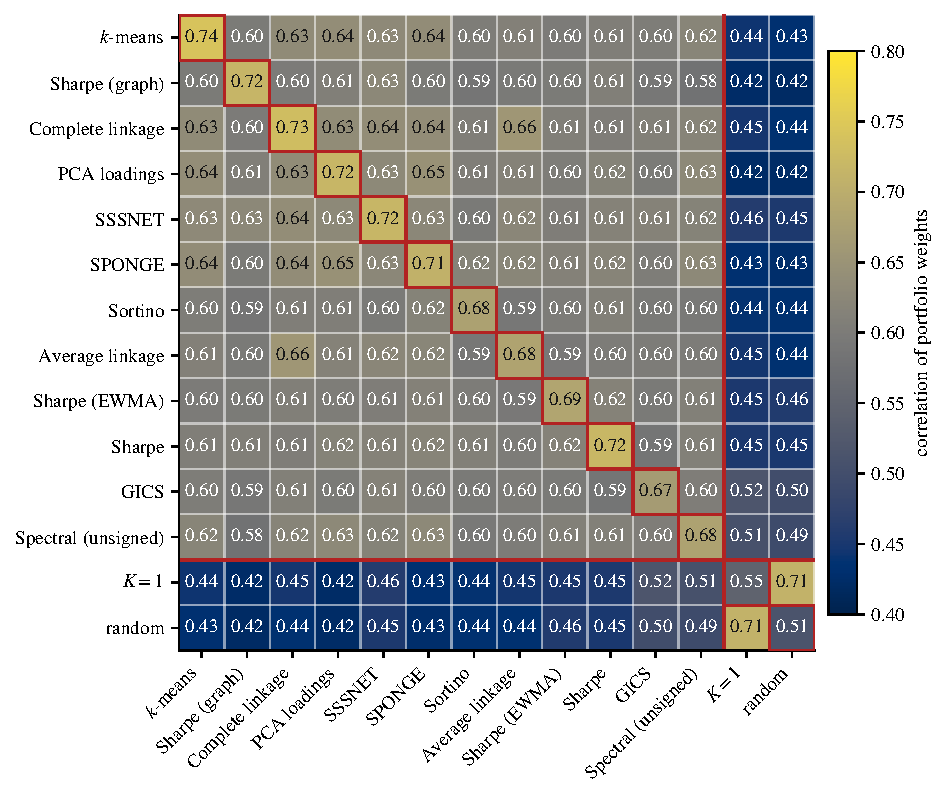
\includegraphics[width=\linewidth]{fig_bet_corr}
\caption{Position-vector correlation between arms. This figure shows the daily position-vector correlation between every pair of the 14 arms at the trained component over the common $6{,}913$-day window, ordered by Sharpe ratio. The diagonal is not one: it is each
arm against itself at a different seed, so every cell can be compared against the diagonal of its own row. The two controls are set off by a
divider line.}
\label{fig:bet_corr}
\end{figure}

The controls give a reference for how low the correlation falls between books that differ in substance. Relative to a clusterizer's correlation with its own refit, $0.704$, the correlation drops by $0.09$ between two clusterizers (to $0.612$) and by $0.25$ between a clusterizer and a control (to $0.450$); the first drop is $36\%$ of the second. The two controls correlate with each other at $0.71$, more than either correlates with its own refit under a redrawn head seed, $0.55$ and $0.51$; every clusterizer's own-refit correlation is $0.67$ to $0.74$. No clustering and a random partition therefore deliver much the same book, and retraining on a structureless signal is noisier than retraining on any partition. The instability is in the fit rather than the partition. The $\K=1$ control has no partition seed to redraw, and the random control's labels carry no structure under any seed, so the random control's Sharpe ratio moves as much when the label stream is redrawn as when the training seed is ($0.39$ across partition draws against $0.41$ across head seeds, \secref{sec:pseed}).

Because the 12 books are this similar, holding all of them at equal weight is as good as selecting among them. The equal-weight book earns a Sharpe ratio of $2.505$ on the seed-averaged payoff, above nine of the 12 books on that convention. Re-selecting the trailing best clusterizer each January leaves a gap to the equal-weight book whose confidence interval covers zero at every look-back considered (\figref{fig:select_vs_ew}). The match between equal weights and selection is the forecast-combination result in trading form: when candidates are exchangeable up to noise, equal weights are hard to beat \citep{timmermann2006forecast}.

Five of the 12 clusterizers, however, sit reliably below the equal-weight book, by $0.17$ to $0.60$ in Sharpe ratio; the intervals are from a circular block bootstrap over days (block $21$, $B = 5{,}000$). One of the five, Sharpe (EW), has a gap of $0.27$ against a range of $0.30$ across its own five partition draws, so its shortfall is not separated from the movement its own partition seed produces; of the other four, two clear their range and two have deterministic partitions and no such range to clear.
Three clusterizers score above the equal-weight book, $k$-means, Sharpe (graph), and complete linkage, by $0.27$, $0.13$, and $0.05$; only $k$-means' interval excludes zero, $[0.10, 0.44]$. Its margin of $0.27$ is about the size of the $0.29$ range its own five partition draws produce, so the one advantage the day bootstrap resolves is not separated from the partition axis. Differences of this size do not identify a best clusterizer. They do identify the clusterizers to avoid, and the clusterizers furthest below the equal-weight book are the most volatile (\secref{sec:hedge}).

\begin{figure}[tb]
\centering
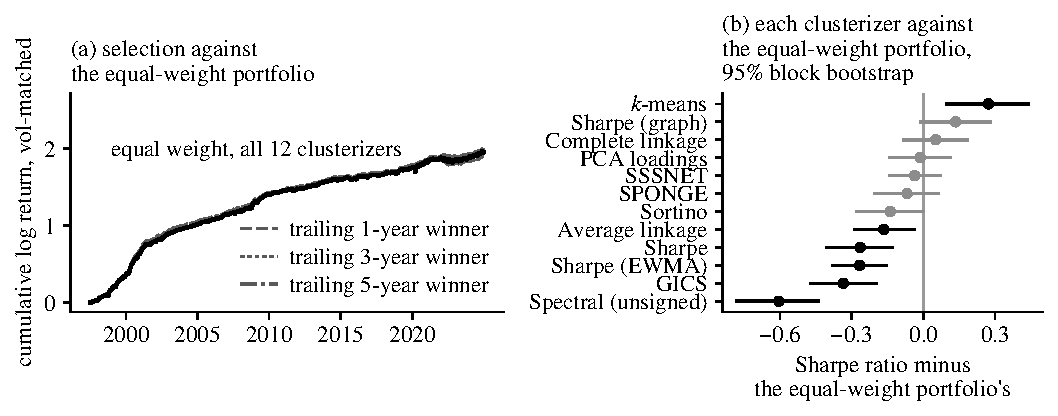
\includegraphics[width=\linewidth]{fig_select_vs_ew}
\caption{Selecting the trailing best clusterizer against holding all 12. This figure plots two comparisons of the seed-averaged trained books. (a) Cumulative log return of the equal-weight book and of three selection rules, each of which re-selects on the first trading day of each calendar year the clusterizer with the highest Sharpe ratio over the trailing one, three, or five years and holds it for the year; series are scaled to equal volatility. (b) Each clusterizer's Sharpe ratio minus the equal-weight book's, with $95\%$ circular block-bootstrap intervals (block $21$, $5{,}000$ draws). All books are seed-averaged trained books over the $6{,}913$-day sample, and panel (b) is ordered by that convention's Sharpe ratio rather than by the mean-of-per-seed ranking of \figref{fig:field_ruler}.}
\label{fig:select_vs_ew}
\end{figure}

%%  ⚠ 5.4 REWRITTEN 2026-08-20 on v3, then CORRECTED the same day after an
%%    adversarial pass. Every number recomputed from source on ALL 6,914
%%    common days (not a sample); script _reference/plot_bet_corr.py.
%%  ⛔ The rule-based POSITIONS row was withdrawn from tab:gradient. The
%%    author's hand-rolled naive book was never validated against the
%%    shipped naive Sharpes and is NOT the engine's book (the engine
%%    carries a 21-day correlation basis, a validity mask and a refit
%%    schedule; p1_lib.naive_stream). Restore the row only from a
%%    reimplementation that reproduces naive_routeA_v3_raw.csv, and
%%    persist the per-day books first -- there is currently no per-day
%%    payoff artifact for ANY v3 rule-based arm.
%%  ⛔ The ceiling footnote is mandatory (top-k exceeds 100%); do not let
%%    an edit turn the ceiling into a bound over all weightings.
%%  ⛔ Do NOT restore "every interval covers zero" as an unqualified claim
%%    about the twelve arms, and do NOT restore the "-0.08 to +0.08"
%%    selection range: that figure came from the v2 caption file and two
%%    independent v3 recomputes disagree with it and with each other.
%%    fig_select_vs_ew must be regenerated on v3 under one documented
%%    selection rule before it ships.
%%  ⚠ tab:onebet (0.87/0.83, PC1 88%/85%, 1.1/1.2 effective bets) was
%%    retired into tab:gradient's last row. v3 seed-averaged trained
%%    equivalents, if a referee wants them: rho-bar 0.866 on twelve,
%%    0.863 on the eleven of tab:gradient; PC1 87.7%.

\subsection{The Estimation Window and the Number of Groups}
\label{sec:window}
Two upstream inputs move the Sharpe ratio on the scale of the span between clusterizers: the length of a clusterizer's estimation window, which moves it by as much as the whole span, and the number of groups $\K$, which moves it by up to $0.36$ away from the $\K = 30$ used throughout, nearly half the span. The comparisons above hold both fixed. Holding the algorithm, the panel, the trading head, and the seeds fixed, we lengthen the window from $21$ days to $252$. Spectral clustering gains $+0.88$ in Sharpe ratio and PCA loadings $+0.66$, each monotone across the intermediate windows and paired by seed, while average linkage, which uses the same correlation matrix, moves $-0.00$. The difference between those responses is the clean comparison, because the arms use the same input; against average linkage, the window response of spectral clustering is $+0.88$ and of PCA loadings $+0.67$, the same sign in every seed. The two clusterizers that gain are the two that use individual eigenvectors of the correlation matrix, and three arms registered in advance to separate that account from its rival (that low starters gain most) move as the eigenvector account predicts (\appref{app:window}).

The number of groups is the second input. Of five clusterizers swept at $\K \in \{10, 30, 50\}$ (five seeds each, \appref{app:ksweep}), three rise monotonically in $\K$, while $k$-means on returns and spectral clustering peak at $30$ and fall by $0.09$ and $0.14$ between $30$ groups and $50$. For the four other than spectral clustering, coarsening to $10$ groups costs $0.20$ to $0.36$ in Sharpe ratio, and refining to $50$ changes it by $-0.09$ to $+0.22$. The gain from more groups cannot be split between finer structure and the finer demeaning of \secref{sec:mechanism} without a random control at each $\K$, which was not run; one run per $\K$ would not suffice (\appref{app:ksweep}). A downstream Sharpe ratio therefore distinguishes changes in the information supplied to the clusterizer and in the number of groups, but discriminates much less sharply among algorithms given the same input.

%% Source: discriminating cells, three seeds each, gate-clean,
%% spot-verified against recomputed SRs 2026-08-16 night:
%% agglo_avg@K10 w21 2.1011 -> w252 2.0873 (delta -0.0138, p=0.80);
%% pca_load@K50 2.0741 -> 2.9842 (+0.9101, p=0.002, CI [0.75,1.07]);
%% random@K30 1.4052 -> 1.3664 (-0.0388, p=0.67). Rival
%% delta = -0.8563*SR_w21 + 2.1866.
%%  ⚠ 5.5 GUARDRAILS (N20/N21):
%%  ⛔ never the t's (68.0, 30.96 -- degenerate denominators); effect
%%     sizes only, as drafted.
%%  ⛔ no "the window moves one rule further than the algorithm moves the
%%     field" -- withdrawn, reverses on 2 of 3 seeds paired.
%%  ⛔ kmeans_ret is NOT a window-unused control (window = its feature
%%     dimension, ARI(w21,w252)=0.143); its delta is "indistinguishable
%%     from zero, CI +/-0.41", not "no effect". Not drafted here at all,
%%     deliberately.
%%  ⛔ sponge +0.41 (p=0.045) left out of the prose: leave-one-seed-out
%%     fails 2 of 3, and its w120/w252 arms carry the GRAPH_LOOKBACK
%%     day-set confound (N22(e)). If an editor wants it, footnote it.
%%  ⚠ the discriminating experiment: first cell landed (agglo_avg@K10
%%     w21 2.1011, separation 0.377 vs sd 0.116) but the outcome cells
%%     had not; nothing printable yet.
%%
%%  ── EXHIBITS FOR THE REMAINING SUBSECTIONS%%
%%  ── EXHIBITS FOR THE REMAINING SUBSECTIONS ──────────────────────────
%%  5.3 formal tests: a TABLE, not a figure — test | question | result:
%%      MCS 90% (T_max) keeps 9/12 | T_R at rule-based keeps 3 | LW 7/66
%%      past Holm, none adjacent | Sortino-vs-Sharpe twin +0.0874
%%      (s.e. 0.0989) | non-overlapping 21-day sums: spread 0.5522 ->
%%      0.2155, 75% MCS keeps all twelve, 0/66.
%%      ⚠ ALL on the OLD mixed-window set — name it in the caption, and a
%%      matched-field recompute is on request to the compute branch.
%%  5.4 one bet in twelve costumes: REUSE fig_cum_pnl (already built —
%%      five arms' cumulative wealth, paths differing in roughness not
%%      drift) + the four numbers rho-bar 0.8325 / breadth 1.18 /
%%      PC1 84.7% / EW 99.17% of ceiling. ⚠ same old-set caveat.
%%  5.5 window: REUSE fig_window_twin (60 vs 21 with seed bands) — its
%%      caption already carries the right reading; add the DiD numbers
%%      (+0.578 / +0.784 vs agglo_avg) and the rival-model concession.
